\documentclass[a4paper,11pt]{article}

\usepackage{../préambule}

\title{Contrôle n°3 : Symétrie}
\date{}
\author{Prénom : {\color{red} CORRECTION}}

\begin{luacode}
dofile "symetrie.lua"
\end{luacode}

\mdfdefinestyle{otherexamplestyle}{
	linecolor=black!70,
    linewidth=1pt,
    backgroundcolor=gray!0,
    frametitlefontcolor=myblue,
    frametitlebackgroundcolor=gray!10,
    frametitlerulecolor=black!30,
	frametitle={Exemple},
	topline=false,
    bottomline=false,
    rightline=false,
	shadow=false,
    leftmargin=12,
    innertopmargin=\topskip,
}

\newmdenv[style=otherexamplestyle]{other_exemple}

\makeatletter
\renewcommand{\maketitle}{%
    \topskip1em
	\@author \hfill \@date \\

	\begin{center}
		\begin{huge}
			\@title \\[1em]
		\end{huge}
	\end{center}
}
\makeatother

\begin{document}

\maketitle

\begin{attention}
	Laisse tes traits de construction.
\end{attention}

\begin{exercice}[(3 points)]\

	Trace le symétrique de la figure par rapport à \myuline{l'axe} $(d)$ :

	\begin{center}
		\begin{tikzpicture}[scale=0.8]
			\directlua{
			local d = {
					p1 = { x = 3.6, y = -0.6 },
					p2 = { x = 10.6, y = 9.9 },
				}
			local points1 = {
			{ x = 3, y = 3 },
			{ x = 2, y = 6 },
			{ x = 4, y = 7 },
			{ x = 6, y = 3 },
			}
			local points2 = {
			{ x = 3, y = 3 },
			{ x = 5, y = 5 },
			{ x = 8, y = 6 },
			}
			local points3 = {
			{ x = 4, y = 7 },
			{ x = 8, y = 6 },
			}
			tikz_draw_points(points1, "thick")
			tikz_draw_points(symetrie_axiale(d, points1), "thick,red")
			tikz_draw_points(points2, "thick")
			tikz_draw_points(symetrie_axiale(d, points2), "thick,red")
			tikz_draw_points(points3, "thick")
			tikz_draw_points(symetrie_axiale(d, points3), "thick,red")
			}
			\coordinate (d1) at (3.6,-0.6);
			\coordinate (d2) at (10.6,9.9);
			\draw[ultra thin] (0,0) grid (14,9);

			\draw[ultra thick] (d1) node[below] {$(d)$} -- (d2);
		\end{tikzpicture}
	\end{center}
\end{exercice}

\begin{exercice}[(3 points)]\

	Trace le symétrique de la figure par rapport \myuline{au point} $C$ : \vspace{1em}

	\begin{center}
		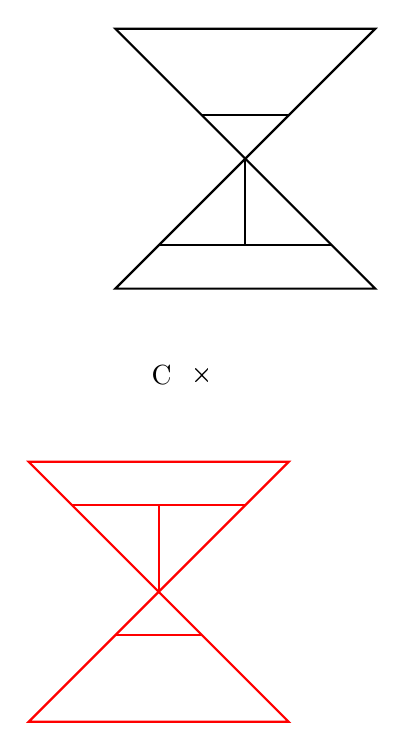
\begin{tikzpicture}[scale=1.1]
			\node[label=left:{C}] (C) at (0,0) {×};

			\draw[thick] (-1,1) -- ++(3,0) -- ++(-3,3) -- ++(3,0) -- cycle;
			\draw[thick] (-0.5,1.5) -- ++(2,0);
			\draw[thick] (1,3) -- ++(-1,0);
			\draw[thick] (0.5,2.5) -- ++(0,-1);

			\draw[thick,red,rotate around={180:(C)}] (-1,1) -- ++(3,0) -- ++(-3,3) -- ++(3,0) -- cycle;
			\draw[thick,red,rotate around={180:(C)}] (-0.5,1.5) -- ++(2,0);
			\draw[thick,red,rotate around={180:(C)}] (1,3) -- ++(-1,0);
			\draw[thick,red,rotate around={180:(C)}] (0.5,2.5) -- ++(0,-1);
		\end{tikzpicture}
	\end{center}
\end{exercice}

\newpage

\begin{exercice}[(4 points)] \

	\begin{attention}
		Ceci est un questionnaire à choix multiples. Pour chaque énoncé, \textbf{\myuline{plusieurs}} \textbf{\myuline{réponses}} sont possibles. \\[0.5em]
		Note tes réponses en dessous de la grille. \\[0.5em]
		Aucune justification n'est demandée.

		\begin{other_exemple}
			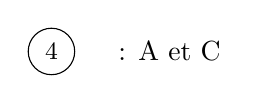
\begin{tikzpicture}
				\node[draw=black,circle] at (0,0) {\small 4};
				\node at (1.5,0) {: A et C};
			\end{tikzpicture}
		\end{other_exemple}
	\end{attention}

	\renewcommand{\arraystretch}{1.3}
	\hspace*{-1.5cm}\begin{tabular}{|p{4cm}|p{3cm}|p{3cm}|p{3cm}|p{3cm}|}
		\hline
		\rowcolor{gray!70}	Enoncés  & réponse A & réponse B & réponse C & réponse D \\ \hline
		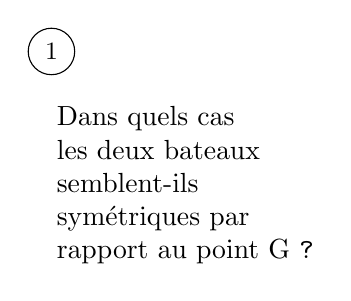
\begin{tikzpicture}
			\node[draw=black,circle] at (-1.7,1.7) {\small 1};
			\node[align=left] at (0,0) {Dans quels cas \\ les deux bateaux \\ semblent-ils \\ symétriques par \\ rapport au point G \verb|?|};
		\end{tikzpicture}
		                           &
		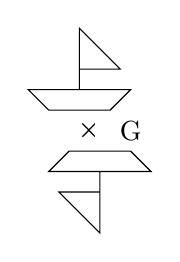
\begin{tikzpicture}[scale=0.26]
			\node[label=right:{G}] (G) at (0,0) {×};
			\draw (-2,1) -- ++(3,0) -- ++(1,1) -- ++(-2.5,0) -- ++(0,3) -- ++(2,-2) -- ++(-2,0) ++(0,-1) -- ++(-2.5,0) -- ++(1,-1);
			\draw[rotate around={180:(G)}] (-2,1) -- ++(3,0) -- ++(1,1) -- ++(-2.5,0) -- ++(0,3) -- ++(2,-2) -- ++(-2,0) ++(0,-1) -- ++(-2.5,0) -- ++(1,-1);
		\end{tikzpicture}  &
		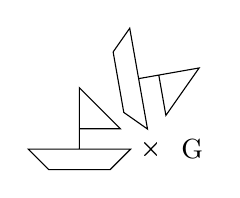
\begin{tikzpicture}[scale=0.26]
			\node[label=right:{G}] (G) at (0,0) {×};
			\draw (-5,-1) -- ++(3,0) -- ++(1,1) -- ++(-2.5,0) -- ++(0,3) -- ++(2,-2) -- ++(-2,0) ++(0,-1) -- ++(-2.5,0) -- ++(1,-1);
			\draw[rotate around={280:(G)}] (-5,-1) -- ++(3,0) -- ++(1,1) -- ++(-2.5,0) -- ++(0,3) -- ++(2,-2) -- ++(-2,0) ++(0,-1) -- ++(-2.5,0) -- ++(1,-1);
		\end{tikzpicture}  &
		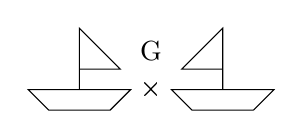
\begin{tikzpicture}[scale=0.26]
			\node[label=above:{G}] (G) at (0,0) {×};
			\draw (-5,-1) -- ++(3,0) -- ++(1,1) -- ++(-2.5,0) -- ++(0,3) -- ++(2,-2) -- ++(-2,0) ++(0,-1) -- ++(-2.5,0) -- ++(1,-1);
			\begin{scope}[yscale=1,xscale=-1]
				\draw (-5,-1) -- ++(3,0) -- ++(1,1) -- ++(-2.5,0) -- ++(0,3) -- ++(2,-2) -- ++(-2,0) ++(0,-1) -- ++(-2.5,0) -- ++(1,-1);
			\end{scope}
		\end{tikzpicture} &
		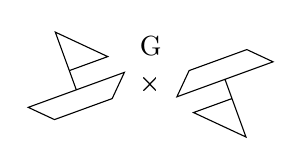
\begin{tikzpicture}[scale=0.26]
			\node[label=above:{G}] (G) at (0,0) {×};
			\draw[rotate around={20:(G)}] (-5,0) -- ++(3,0) -- ++(1,1) -- ++(-2.5,0) -- ++(0,3) -- ++(2,-2) -- ++(-2,0) ++(0,-1) -- ++(-2.5,0) -- ++(1,-1);
			\draw[rotate around={200:(G)}] (-5,0) -- ++(3,0) -- ++(1,1) -- ++(-2.5,0) -- ++(0,3) -- ++(2,-2) -- ++(-2,0) ++(0,-1) -- ++(-2.5,0) -- ++(1,-1);
		\end{tikzpicture}                                                  \\ \hline
		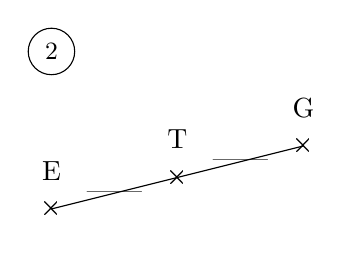
\begin{tikzpicture}[scale=0.8]
			\node[draw=black,circle] at (-2,2) {\small 2};

			\coordinate (E) at (-2,-0.5);
			\coordinate (T) at (0,0);
			\coordinate (G) at (2,0.5);
			\node[label=above:{T}] at (T) {×};
			\node[label=above:{E}] at (E) {×};
			\node[label=above:{G}] at (G) {×};

			\draw (E) -- node{||} (T);
			\draw (T) -- node{||} (G);
		\end{tikzpicture} &
		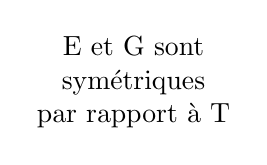
\begin{tikzpicture}
			\node[align=center] at (0,0) {E et G sont \\ symétriques \\ par rapport à T};
		\end{tikzpicture} &
		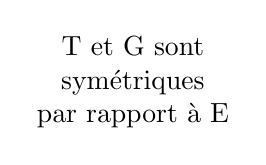
\begin{tikzpicture}
			\node[align=center] at (0,0) {T et G sont \\ symétriques \\ par rapport à E};
		\end{tikzpicture} &
		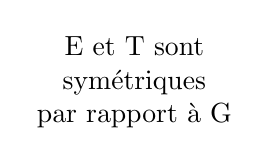
\begin{tikzpicture}
			\node[align=center] at (0,0) {E et T sont \\ symétriques \\ par rapport à G};
		\end{tikzpicture} &
		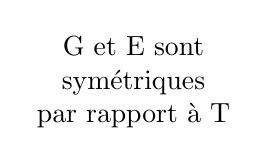
\begin{tikzpicture}
			\node[align=center] at (0,0) {G et E sont \\ symétriques \\ par rapport à T};
		\end{tikzpicture}                                                 \\ \hline
		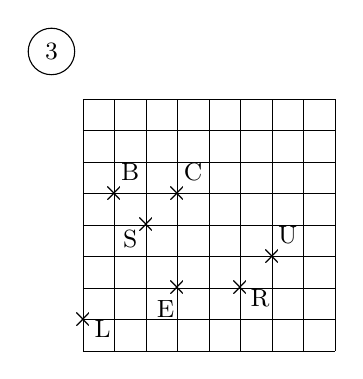
\begin{tikzpicture}[scale=0.4]
			\node[draw=black,circle] at (-1,9.5) {\small 3};
			\draw[ultra thin] (0,0) grid (8,8);
			\coordinate (L) at (0,1);
			\coordinate (S) at (2,4);
			\coordinate (B) at (1,5);
			\coordinate (C) at (3,5);
			\coordinate (E) at (3,2);
			\coordinate (U) at (6,3);
			\coordinate (R) at (5,2);

			\node[label={[xshift=0.25cm, yshift=-0.6cm]\small L}] at (L) {×};
			\node[label={[xshift=-0.2cm, yshift=-0.65cm]\small S}] at (S) {×};
			\node[label={[xshift=0.2cm, yshift=-0.2cm]\small B}] at (B) {×};
			\node[label={[xshift=0.2cm, yshift=-0.2cm]\small C}] at (C) {×};
			\node[label={[xshift=-0.15cm, yshift=-0.75cm]\small E}] at (E) {×};
			\node[label={[xshift=0.2cm, yshift=-0.2cm]\small U}] at (U) {×};
			\node[label={[xshift=0.25cm, yshift=-0.6cm]\small R}] at (R) {×};
		\end{tikzpicture} &
		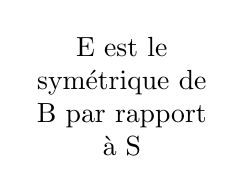
\begin{tikzpicture}
			\node[align=center] at (0,0) {E est le \\ symétrique de \\ B par rapport \\ à S};
		\end{tikzpicture} &
		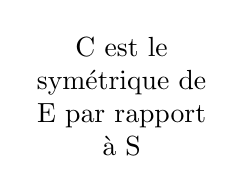
\begin{tikzpicture}
			\node[align=center] at (0,0) {C est le \\ symétrique de \\ E par rapport \\ à S};
		\end{tikzpicture} &
		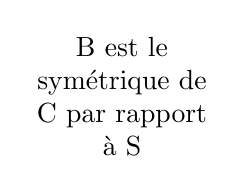
\begin{tikzpicture}
			\node[align=center] at (0,0) {B est le \\ symétrique de \\ C par rapport \\ à S};
		\end{tikzpicture} &
		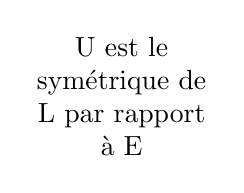
\begin{tikzpicture}
			\node[align=center] at (0,0) {U est le \\ symétrique de \\ L par rapport \\ à E};
		\end{tikzpicture}                                                 \\ \hline
	\end{tabular} \vspace{2em}

	\begin{tikzpicture}
		\node[draw=black,circle] at (0,0) {\small 1};
		\node at (2,0) {: {\color{red} A et D}};
		\node[draw=black,circle] at (0,-2) {\small 2};
		\node at (2,-2) {: {\color{red} A et D}};
		\node[draw=black,circle] at (0,-4) {\small 3};
		\node at (1.5,-4) {: {\color{red} D}};
	\end{tikzpicture}
\end{exercice}

\end{document}